% tikzpic.tex
\documentclass[crop,tikz]{standalone}% 'crop' is the default for v1.0, before it was 'preview'
%\usetikzlibrary{...}% tikz package already loaded by 'tikz' option
\usepackage{amsmath,amssymb}
\usetikzlibrary{arrows, positioning}
\usepackage[T1]{fontenc}
\begin{document}
    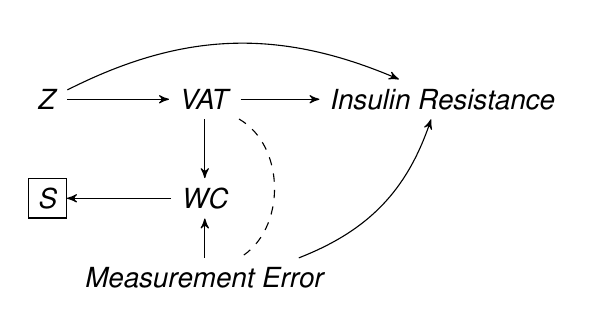
\begin{tikzpicture}
	[->,>=stealth', auto, node distance=2cm,main node/.style={circle,draw,font=\sffamily\Large}]
	%\begin{scope}
	\node (L)[font=\fontfamily{phv}\selectfont] {\textit{Z}};
	\node (A) [font=\fontfamily{phv}\selectfont, right of = L] {\textit{VAT}};
	\node (Y) [font=\fontfamily{phv}\selectfont, right = 1 cm of A] {\textit{Insulin Resistance}};
	\node (As) [font=\fontfamily{phv}\selectfont, below = 0.75cm of A] {\textit{WC}};
	\node (eps) [font=\fontfamily{phv}\selectfont, below = 0.5cm of As] {\textit{Measurement Error}};
	\node (S) [font=\fontfamily{phv}\selectfont, draw, below = 0.75cm of L] {\textit{S}};
	\path[every node/.style={font=\sffamily\small}]
	(A) edge node [right] {} (Y)
	(L) edge [bend left = 25] node [right] {} (Y)
	(L) edge node [right] {} (A)
	(A) edge node [right] {} (As)
	(eps) edge node [right] {} (As)
	(eps) edge [bend right = 25] node [right] {} (Y)
	(As) edge node [right] {} (S);
	\path (A) [-,dashed, bend left = 60] edge (eps);
\end{tikzpicture}
\end{document}